\documentclass[11pt,letterpaper]{article}
% --- Packages ---
\usepackage[utf8]{inputenc}
\usepackage[margin=1in]{geometry}
\usepackage{amsmath, amssymb, amsthm, amsfonts}
\usepackage{graphicx}
\usepackage{xcolor}
\usepackage{hyperref}
\usepackage{booktabs}
\usepackage{cite}
\usepackage{microtype}
\usepackage{titlesec}
\usepackage{tcolorbox}
\usepackage{enumitem}
\usepackage{longtable}
\usepackage{booktabs}
% --- Color Palette (De-saturated, Academic & Professional) ---
\definecolor{ajpblue}{RGB}{28, 54, 115}   % Deep navy accent
\definecolor{ajpsec}{RGB}{54, 95, 145}   % Secondary slate blue
\definecolor{bglight}{RGB}{245, 247, 250} % Light background for callout boxes
\definecolor{bordergrey}{RGB}{210, 215, 223}
% --- Hyperref Setup ---
\hypersetup{
colorlinks=true,
linkcolor=ajpblue,
citecolor=ajpsec,
urlcolor=ajpblue
}
% --- Typography & Headings Styling ---
\titleformat{\section}{\large\bfseries\color{ajpblue}}{\thesection}{1em}{}[{\titlerule[0.5pt]}]
\titleformat{\subsection}{\normalsize\bfseries\color{ajpsec}}{\thesubsection}{1em}{}
% --- Custom Environments for Explanation ---
\newtcolorbox{equationbreakdown}[1]{
colback=bglight,
colframe=ajpblue,
fonttitle=\bfseries,
title={Derivation Details \& Interpretation: #1},
arc=3pt,
boxrule=1pt,
bottomtitle=2mm,
toptitle=2mm
}
\newtcolorbox{physicsinsight}{
colback=bglight,
colframe=ajpsec,
boxrule=0.5pt,
left=4mm,
right=4mm,
top=3mm,
bottom=3mm,
arc=2pt,
}
% --- Title & Project Metadata ---
\title{
\vspace{-1.5in}
\rule{\linewidth}{1.5pt} \\ \vspace{4mm}
\large\textbf{PHYSICS GROUP PROJECT REPORT} \\ \vspace{2mm}
\Large\textbf{An Explanatory Guide and Step-by-Step
Derivation of: \\ ``[ Sling Internal Ballistics ]''}
\\ \vspace{4mm}
\large\textit{Based on the Article in the American Journal of
Physics} \\
\rule{\linewidth}{1.5pt}
}
% Multi-column author format for a group project
\author{
\begin{tabular}{r @{\quad} l}
\textbf{Project Group:} & [New Group 12 / Team
JPS] \\[1ex]
\textbf{Group Members:} & HyeRim Jung(202611202)\\
& BoRa Shim(202611120), SoJin Park(202611088), HeeJee Jang(202611191)\\
\textbf{Instructor:}    & Dr. Professor Deniz Olgu Devecioglu \\
\textbf{Department:}    & Department of Physics, DGIST
\end{tabular}
} 
\date{\today}
\begin{document}
\maketitle
\begin{abstract}
This project provides a comprehensive, pedagogical breakdown
of the foundational paper \textbf{``[Sling Internal Ballistics]''} by
[Mark Denny], published in the \textit{American
Journal of Physics} (\textbf{Issue}, Page Start-Page End, 2025)
\cite{originalpaper}. While the original text assumes a
certain level of mathematical and physical maturity, this
report fills in the intermediate algebraic steps, explains
the contextual physics principles, and interprets key
equations. We reconstruct the derivations of the central
models, analyze physical approximations, and discuss the
implications of the results.
\end{abstract}
\tableofcontents

% =========================================================================
\section{Introduction \& Contextual Background}
% =========================================================================
To understand motion, we often simplify complex structures and set idealized models. The basic motion obtained through this simplification becomes the basis for understanding and analyzing real motion. In this paper, we review Section II of Internal Ballistics of the Sling to examine rotational dynamics and to explore the approximation as a powerful tool for understanding it.
\subsection{Historical and Pedagogical Significance}
This paper reviews the physical analysis of \textbf{"[sling internal ballistics]"} by [Mark DEnny], published in the \textit{American Journal of Physics}, with particular focus on the introductory framework and the pirouette-style model presented in Sections I and II of Mark Denny’s Internal Ballistics of the Sling. The original paper investigates the motion of a sling bullet before release, a phase known as internal ballistics, and emphasizes that the complexity of sling motion requires carefully chosen physical approximations. In Section I, the sling is introduced as an ancient projectile weapon whose internal dynamics involve three-dimensional motion, precise release timing, and significant bullet spin. Section II simplifies this complex motion by considering the pirouette style, in which the slinger and sling rotate in a manner similar to an Olympic hammer thrower. Using this model, the release velocity is estimated from rotational motion, mechanical power transfer, sling length, projectile mass, and the number of rotations prior to release. This review highlights how simplified assumptions, such as neglecting gravity and air resistance during the short internal phase, allow a complicated real-world motion to be understood through basic rotational dynamics. Overall, the analysis demonstrates the educational value of approximation in the application of physics to historical projectile motion.
\subsection{Physical Setup and System Parameters}
In the original paper, the slinger and the sling rotate in a manner similar to a hammer thrower. The sling bullet is approximated to move along a circular arc of fixed
radius $r$, where $r$ represents the distance from the rotation axis to the bullet. The bullet completes $n$ rotations before release, and the angular motion is modeled using a constant angular acceleration $\alpha$.
This simplified setup reduces the sling's complex internal motion to planar circular motion. After release, the bullet is treated as a projectile, so its range can be estimated with and without air resistance.
Table~\ref{tab:variables}.
\begin{longtable}{lll}
\caption{Key Symbols, Constants, and Variables used in the Analysis.}
\label{tab:variables}\\

\toprule
\textbf{Symbol} & \textbf{Physical Meaning} & \textbf{SI Units} \\
\midrule
\endfirsthead

\caption[]{Key Symbols, Constants, and Variables used in the Analysis. (continued)}\\
\toprule
\textbf{Symbol} & \textbf{Physical Meaning} & \textbf{SI Units} \\
\midrule
\endhead

\midrule
\multicolumn{3}{r}{\textit{Continued on next page}}\\
\endfoot

\bottomrule
\endlastfoot

$m$ & Mass of the sling bullet & $\mathrm{kg}$ \\
$r$ & Radius of circular motion, arm length plus sling length & $\mathrm{m}$ \\
$n$ & Number of rotations before release & dimensionless \\
$\theta$ & Angular position of the bullet & $\mathrm{rad}$ \\
$\alpha$ & Constant angular acceleration & $\mathrm{rad/s^2}$ \\
$t_n$ & Time required for $n$ rotations & $\mathrm{s}$ \\
$v$ & Release speed of the bullet & $\mathrm{m/s}$ \\
$P_n$ & Average mechanical power transferred to the bullet & $\mathrm{W}$ \\
$R$ & Projectile range & $\mathrm{m}$ \\
$\gamma$ & Launch angle above the horizontal & $\mathrm{rad}$ or degree \\
$W$ & Target width & $\mathrm{m}$ \\
$\Delta t$ & Maximum tolerable release timing error & $\mathrm{s}$ \\
$f$ & Bullet spin frequency & $\mathrm{Hz}$ \\

\end{longtable}
% =========================================================================
\section{Step-by-Step Mathematical Derivations}
% =========================================================================

\subsection{The Starting Framework (Original Equation 1)}
\begin{equation}
v = 2(\pi r \frac{n\bar{P_n}}{m})^\frac{1}{3}
\end{equation}

\subsection{Filling in the Missing Steps}
When the bullet moves around a circle $n$ times before release. let $\ddot{\theta} = \alpha$. It is released after moving an angle $\theta_n = 2n\pi = \alpha t^2/2$. Since the bullet is modeled as moving along a circular arc of radius $r$, its instantaneous linear speed equals the tangential speed in circular motion. Therefore, at the moment of release, the launch speed is $v=\ddot{\theta}r$

\begin{align*}
    \ddot{\theta}=\alpha ,\ \dot{\theta}&=\alpha t ,\ \theta = \frac{1}{2}\alpha t^2\\
    \theta_n = &2n\pi = \frac{1}{2}\alpha t_n^2\\[0.5em]
    t_n^2 &= \frac{4n\pi}{\alpha}\\
\end{align*}
Therefore, the release speed is\\
\begin{equation}
t_n = 2\sqrt{\frac{n\pi}{\alpha}}
\end{equation}
Using Eq. (2), we can express $\dot{\theta}$ as follows.\\
\begin{align*}
\ \dot{\theta_n} &= \alpha t_n\\
&= \alpha\times 2\sqrt{n\pi\over{\alpha}}\\[0.5em]
&= 2\sqrt{n\pi\alpha}
\end{align*}
Therefore, $\theta_n$ is
\\
\begin{equation}
\dot\theta_n = 2\sqrt{n\pi\alpha}
\end{equation}
\\
Then, we combine Eq. (2) with $v=\dot{\theta} r$.
\begin{align*}
v 
&= r \times 2\sqrt{n\pi \alpha}\\[0.5em]
&= 2r\sqrt{n\pi\alpha}
\end{align*}

\begin{equation}
v = 2r\sqrt{n\pi\alpha}
\end{equation}
\\
Let us average power to $\bar{P}$,
\begin{align*}
\bar{P_n}&=\frac{E}{t}=\frac{mv^2}{2t}
\end{align*}
Using Eq. (2), we can also express $\bar{P_n}$ as follows.\\
\begin{align*}
\bar{P_n}
&=\frac{m\sqrt{\alpha}v^2}{4\sqrt{n\pi}}\\[0.5em]
&=\frac{m\sqrt{\alpha}\times 4r^2 n\pi\alpha}{4\sqrt{n\pi}}\\[0.5em]
&=m\sqrt{\alpha}r^2\sqrt{n\pi\alpha}\\[0.5em]
&=mr^2(n\pi)^\frac{1}{2} \alpha ^\frac{3}{2}
\end{align*}
\\
Therefore, the $\bar{P_n}$ is
\begin{equation}
\bar{P_n}=mr^2(n\pi)^\frac{1}{2} \alpha ^\frac{3}{2}
\end{equation}

\begin{align*}
\alpha ^\frac{3}{2} &= \frac{P_n}{mr^2\sqrt{{n\pi}}}\\[0.5em]
\alpha &= (\frac{P_n}{mr^2\sqrt{n\pi}})^\frac{2}{3}\\[0.5em]
\end{align*}
Let's using Eq. (4) to express $v$
\begin{align*}
v &= 2rn^\frac{1}{2}\pi^\frac{1}{2}\alpha^\frac{1}{2}\\
&= 2rn^\frac{1}{2}\pi^\frac{1}{2}\times(\frac{P_n}{mr^2\sqrt{n\pi}})^\frac{1}{3}\\[0.5em]
&= 2(\frac{rn\pi P_n}{m})^\frac{1}{3}
\end{align*}
\\
Therefore, the $v$ is
\begin{equation*}
v = 2(\pi r \frac{nP_n}{m})^\frac{1}{3}
\end{equation*}
\begin{equationbreakdown}{Release Speed in the Pirouette Model}
\begin{equation*}
v = 2\left(\frac{\pi r n P_n}{m}\right)^{1/3}
\end{equation*}
\\
This is the central result of the pirouette-style model. It connects
the release speed to the average mechanical power transferred by the
slinger, rather than to the detailed motion of the arm and body.
\end{equationbreakdown}

\subsection{The Starting Framework (Original Equation 2)}
\begin{equation}
f \approx \frac{v}{\sqrt{2\pi rb}}
\end{equation}
\subsection{Filling in the Missing Steps}
We approximate the force acting on the bullet by $F_c$, as shown below.\\
\begin{equation}
F_c = \frac{mr^2}{r}\\
\end{equation}
\\
We model the bullet as an elongated ellipsoid and set its moment of inertia about the rotation axis as follows. When the major axis of the ellipsoid is denoted by $a$ and the minor axis by $b$\\
\begin{equation}
\\
I = \frac{m(a^2+b^2)}{5}\\
\end{equation}
\begin{align*}
\tau = b&F_c = I\dot{w}\\[0.5em]
\tau = b\frac{mv^2}{r} &= \dot{w}\frac{m(a^2+b^2)}{5}\\
\end{align*}
By rearranging this expression, we obtain
\begin{align*}
\dot{w}&=\frac{5bv^2}{(a^2+b^2)r}
\end{align*}
If we assume that $a=2b$
\begin{align*}
a &= 2b,\\[0.5em]
\dot{w}&=\frac{v^2}{rb}\\
\end{align*}
When we assume that the bullet has nearly no initial rotation and moves with constant angular acceleration, the bullet's angular position $\phi$ can be written as follows.
\begin{equation}
\Delta \phi = \frac{1}{2}\dot{w}(\Delta t)^2
\end{equation}
\begin{align*}
\frac{1}{2}\dot{w}(\Delta t)^2 &\approx \pi\\[1em]
\dot{w}(\delta t)^2 \approx & \;2\pi\\[0.5em]
(\Delta t)^2 \approx&\,\frac{2\pi}{\dot{w}}
\end{align*}
By rearranging this expression, we obtain
\begin{equation}
\Delta t \approx \sqrt{\frac{2\pi}{\dot{w}}}
\end{equation}
Using $\dot{w} = \frac{v^2}{rb}$, we can rearrange the expression as follows.
\begin{align*}
\Delta t \approx \sqrt{\frac{2\pi rb}{v^2}}
\end{align*}
The frequency satisfies the following relation.
\begin{align*}
f &= \frac{1}{T} = \frac{w}{2\pi}
\end{align*}
When we express the angular velocity with respect to time, we obtain the following expression.
\begin{align*}
w &= \dot{w}\delta t
\end{align*}
Thus, the expression can be written as follows.
\begin{align*}
f &= \frac{\dot{w}\delta t}{2\pi}\\
&\approx \frac{\frac{v^2}{rb} \times \sqrt{\frac{2\pi rb}{v^2}}}{2\pi}\\ &\approx \frac{v}{\sqrt{2\pi rb}}
\end{align*}
\begin{equationbreakdown}{Origin of Bullet Spin}
The high spin rate of the sling bullet comes from the torque exerted
by the pouch during the very short interval after the release cord is
let go. Approximating this force as \(F_c = mv^2/r\) and assuming that
the bullet disengages after about half a rotation gives
\begin{equation}
f \approx \frac{v}{\sqrt{2\pi rb}}
\end{equation}
Thus, faster release speeds and smaller bullets naturally lead to
larger spin rates.
\end{equationbreakdown}



\subsection{The Starting Framework (Original Equation 3)}

\begin{equation}
\Delta t = Wr\sqrt{\frac{sin2\gamma}{4gR^3}}
\end{equation}

\subsection{Filling in the Missing Steps}
When the sling bullet is released, it moves in the tangential direction of the circular path. If the target is located at a distance R and its width is $W$, When the bullet is directed toward the center of the target, the allowable error for hitting the target is $\frac{W}{2}$, which is half of the target width. Therefore, we can approximate the angular error of the launch direction as follows.
\begin{align*}
\\
\Delta\theta\approx \frac{\frac{W}{2}}{R}\\[0.5em]
\Delta\theta= \frac{\frac{W}{2}}{R}\\
\end{align*}
Let us denote the possible error in the exact time at which the bullet should be released by $\Delta t$. Since the sling bullet is in circular motion just before release, we can express it as follows from the relation between tangential velocity and angular velocity.
\begin{align*}
\dot{\theta}&=\frac{v}{r}
\end{align*}
Therefore, the angular position changes with time as follows, and by using $\dot{\theta}=\frac{v}{r}$, we can express it in the following form.
\begin{align*}
\Delta\theta&=\dot{\theta}\Delta t\\
\Delta\theta&=\frac{v}{r}\Delta t
\end{align*}
\begin{align*}
\Delta\theta = \frac{W}{2R}\\[0.5em]
\Delta\theta = \frac{v}{r}{\Delta t}
\end{align*}
In the maximum error condition, the allowable error and the error caused by the release time error must be equal.
\begin{align*}
\frac{v}{r}\Delta t= \frac{W}{2R}
\end{align*}
Then, we obtain the following result.
\begin{equation}
\Delta t = \frac{Wr}{2Rw}\\[0.5em]
\end{equation}
Neglecting air resistance and assuming that the bullet is launched and lands at the same height, the projectile range is approximated as follows.
\begin{equation}
R = \frac{v^2}{g}sin2\gamma
\end{equation}
\begin{align*}
v^2 = \frac{gR}{sin2\gamma}\\[0.5em]
v=\sqrt{\frac{gR}{sin2\gamma}}
\end{align*}
Then, by substituting this result into Eq. (13), we obtain Eq. (12).
\begin{align*}
\Delta t &= \frac{Wr}{2Rv}\\[0.5em]
\Delta t &= \frac{Wr}{2R}\times\sqrt{\frac{sin2\gamma}{gR}}\\[0.5em]
\Delta t &= Wr\sqrt{\frac{sin2\gamma}{4gR^3}}
\end{align*}

\begin{equationbreakdown}{Why Slinging Requires Precise Timing}
A small timing error changes the angular direction of release:
\[
    \Delta \theta = \frac{v}{r}\Delta t.
\]
To hit a target of width \(W\) at range \(R\), this angular error must
be smaller than
\[
    \Delta \theta = \frac{W}{2R}.
\]
Thus,
\[
    \Delta t = \frac{Wr}{2Rv}.
\]

The allowed timing error becomes extremely small for distant targets.
This explains why accurate slinging requires millisecond-level release
control.
\end{equationbreakdown}
% =========================================================================
\section{Physical Approximations and Limiting Cases}
% =========================================================================
\textbf{Section II} of Internal Ballistics of the Sling discusses the pirouette style, a simplified rotational model used to analyze the sling motion more easily. The motion of the sling is considered in terms of release speed, range, and spin of the bullet. Before reviewing the calculations in the paper and conducting an additional experiment, we first introduce the assumptions used and explain their physical meanings. In this paper, they used 5 assumptions.
\begin{enumerate}[label=A\arabic*.]
    \item \textbf{The slinger's arm accelerates at a constant angular rate.}
    
    This assumption simplifies the derivation of the release speed. 
    Although the actual angular acceleration of a slinger is not exactly constant, 
    assuming constant angular acceleration allows the angular velocity and 
    release time to be written in a simple analytic form. In the paper, this 
    assumption is not essential, but it streamlines the calculation and presentation.
\newpage    
    \item \textbf{The small effect of gravity on internal ballistics is ignored.}
    
    During the internal ballistic phase, the bullet is mainly accelerated by the 
    rotational motion of the sling. The gravitational energy is much smaller than 
    the rotational kinetic energy, so gravity has only a small effect on the 
    internal motion. Therefore, gravity is neglected when deriving the release 
    speed, although it is still important after the bullet is released.
    
    \item \textbf{The sling cords are considered to be stiff and massless. Initially, only mechanical power is considered.}
        
    The sling cords are assumed not to stretch and not to contribute significantly 
    to the total mass. As a result, the calculation focuses on the mechanical 
    energy transferred from the slinger to the bullet. The biochemical power of 
    the slinger and the energy needed to move the sling cords themselves are not 
    included in the simplified model.

\begin{physicsinsight}
\textbf{Physical Conceptualization:} 
\\
A3 assumes that the sling cords are stiff and massless. The massless condition can be written as
\[
    m_{\mathrm{cord}} \approx 0,
\]
so the cord's kinetic energy is neglected:
\[
    E_{\mathrm{total}}
    = E_{\mathrm{bullet}} + E_{\mathrm{cord}}
    \approx E_{\mathrm{bullet}}.
\]
With gravity neglected during internal ballistics, this gives
\[
    E_{\mathrm{bullet}} \approx \frac{1}{2}mv^2,
\]
and therefore
\[
    P_n \approx \frac{mv^2}{2t_n}.
\]

The stiffness condition means that the sling radius remains constant:
\[
    r(t)=r, \qquad \dot{r}=0.
\]
Thus, the bullet speed is purely tangential:
\[
    v = r\dot{\theta}.
\]
A3 removes this extra complication and makes the release-speed
derivation possible with a simple circular-motion model.
\end{physicsinsight}
\newpage    
    \item \textbf{Air resistance is neglected for internal ballistics, but is taken into account for external motion.}
    
    The internal ballistic phase lasts for a very short time, so the effect of air 
    resistance during the wind-up motion is assumed to be small. However, after 
    release, the bullet travels a much longer distance through the air. Therefore, 
    air resistance is neglected for the internal motion but included when estimating 
    the external trajectory and range.


\begin{physicsinsight}
\textbf{Physical Conceptualization:} 
A4 assumes that air resistance is neglected during internal ballistics,
but included during external motion. During the short wind-up phase, the
release speed is obtained without a drag term:
\[
    P_n \approx \frac{1}{t_n}\left(\frac{1}{2}mv^2\right).
\]
This means that the work done by the slinger is assumed to become mainly
the kinetic energy of the bullet.

After release, the no-drag projectile range is
\[
    R_{\mathrm{vac}}=\frac{v^2}{g}\sin 2\gamma.
\]
However, for external motion, air resistance is no longer negligible.
Using quadratic drag,
\[
    \mathbf{F}_{\mathrm{drag}}
    =
    -\frac{1}{2}\rho C_D A |\mathbf{v}|\mathbf{v},
\]
the equation of motion becomes
\[
    m\ddot{\mathbf{r}}
    =
    -mg\,\hat{\mathbf{y}}
    -\frac{1}{2}\rho C_D A |\mathbf{v}|\mathbf{v}.
\]
\end{physicsinsight}    
Therefore, A4 justifies why the internal release-speed derivation can
remain simple, while the external range calculation must be corrected
for drag. This is also why the no-drag range is larger than the
drag-included range in the computational comparison.
\newpage
    \item \textbf{Simplified internal bullet trajectory, assumed for the most part to be in one plane. Forces and torques that move the bullet out of this plane are neglected here.}
    
    The actual motion of a sling bullet can be three-dimensional because the 
    slinger may rotate the torso, move forward, or change the plane of rotation 
    before release. In this simplified model, however, the bullet's internal 
    trajectory is treated as motion mainly in one plane. Out-of-plane forces and 
    torques are neglected so that the essential relation between average power, 
    sling length, bullet mass, and release speed can be obtained.
\end{enumerate}
\begin{physicsinsight}
\textbf{Physical Conceptualization:} 
Assumption A5 states that the internal trajectory of the sling bullet is
approximated as motion in a single plane. In the pirouette-style model,
this means that the bullet is treated as moving along a circular arc of
radius \(r\), rather than following a fully three-dimensional path. Thus,
the position of the bullet may be represented as
\[
    \mathbf{r}(t) = r\cos\theta(t)\,\hat{\mathbf{x}}
    + r\sin\theta(t)\,\hat{\mathbf{y}},
\]
with no out-of-plane component:
\[
    z(t) = 0.
\]

Under this approximation, the speed of the bullet is simply the
tangential speed,
\[
    v = r\dot{\theta}.
\]
This relation is essential for deriving the release-speed formula and
for connecting timing error to angular error. If the trajectory were
fully three-dimensional, the speed would generally have additional
components,
\[
    v^2 = r^2\dot{\theta}^{\,2} + \dot{z}^{\,2} + \cdots,
\]
and the analysis would no longer reduce to a simple circular-motion
model.
\end{physicsinsight}
Therefore, A5 is not merely a geometric simplification. It is the
assumption that allows the internal ballistic phase to be modeled using
one angular variable \(\theta(t)\). This makes the release speed,
projectile range, spin estimate, and timing-error calculation tractable.
\newpage
% =========================================================================
\section{Computational or Experimental Verification (Optional)}
% =========================================================================
\subsection{Numerical or Experimental Comparison with Analytical Results}
To computationally reproduce the range comparison discussed in the original paper, we implemented a Python script that plots the projectile range as a function of release speed. The script compares two cases: ideal projectile motion without air resistance and projectile motion with drag. For consistency with the representative pirouette-style model, we used $\gamma = 40^\circ,\, r=2.5\mathrm{m}$, and $n=3$ rotations.
\\
\begin{figure}[h!]
\centering
%\includegraphics[width=0.6\linewidth]{resonance_plot.png} %
% Uncomment and change the file name when image exists
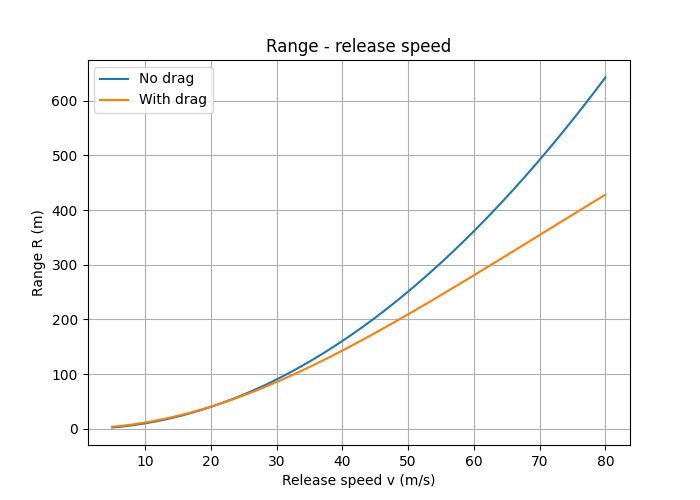
\includegraphics[width=0.8\linewidth]{reproduction of paper.png}
\caption{Python-generated reproduction of the range comparison discussed in Section II.B. 
The no-drag curve follows the ideal projectile model, while the drag-included curve 
shows the reduction of range caused by air resistance during external flight.}
\label{fig:range_drag_comparison}
\end{figure}
\subsection{Interactive VPython Simulation}
In addition to the static Python plot, we developed an interactive
VPython simulation to visualize the pirouette-style sling motion. The simulation allows the user to vary parameters such as average power, bullet mass, sling radius, number of rotations, shoulder height, bullet radius, and sling plane tilt.
\newpage
\begin{figure}
    \centering
    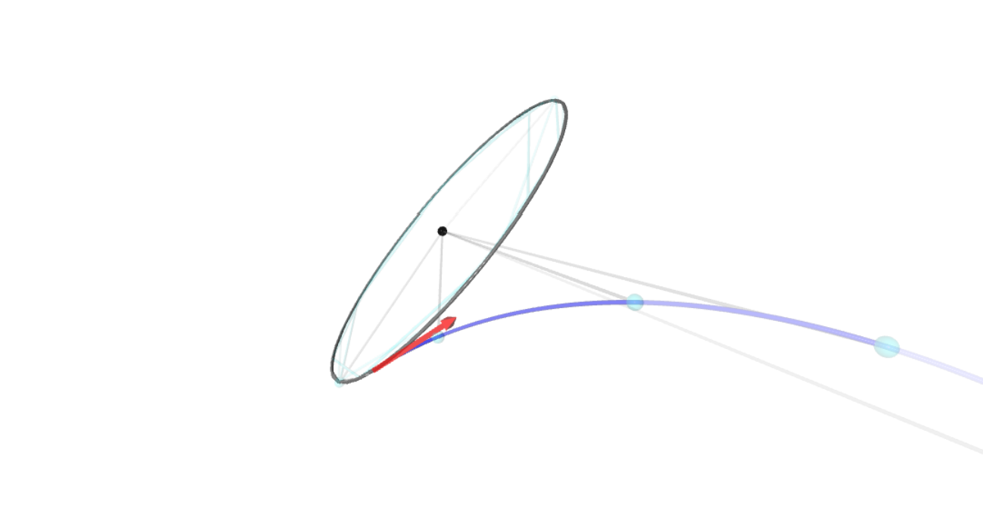
\includegraphics[width=0.5\linewidth]{시뮬레이션 궤적만.png}
    \caption{Interactive VPython simulation of the pirouette-style sling. The model visualizes the internal circular motion and post-release trajectory, along with the corresponding release speed, range, spin rate, and timing error.}
    \label{fig:vpython_pirouette}
\end{figure}
\begin{figure}
    \centering
    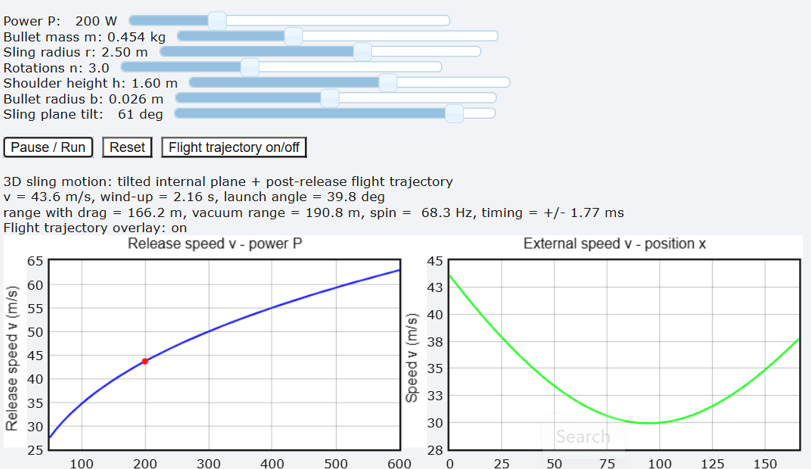
\includegraphics[width=0.5\linewidth]{시뮬레이션 툴.png}
    \caption{The simulation allows the user to adjust the controllers and observe the launch trajectory under different physical conditions.}
    \label{fig:placeholder}
\end{figure}

\subsection{Discussion of Computational Results}

The computational results support the main physical interpretation of
Section II. The Python range comparison shows that the ideal no-drag
model overestimates the projectile range. In the no-drag case, the
bullet is affected only by gravity after release, so the range is given
by the standard projectile equation
\[
    R_{\mathrm{vac}} = \frac{v^2}{g}\sin 2\gamma .
\]
However, when air resistance is included, the drag force continuously
reduces the projectile speed during flight. As a result, the
drag-included range is shorter than the vacuum range. This agrees with
the paper's conclusion that air resistance may be neglected during the
short internal ballistic phase, but it becomes important during the
external ballistic phase.

The VPython simulation provides a complementary visualization of the
same physical model. Instead of only plotting the final range, the
simulation displays the internal circular motion before release and the
external trajectory after release. It also calculates important
quantities such as release speed, range with drag, vacuum range, spin
rate, and release timing error. Therefore, the VPython model helps
connect the analytical equations to the actual motion of the sling
bullet in a more intuitive way.

Both computational implementations should be interpreted as simplified
models rather than complete reproductions of real sling motion. The real
motion of a sling can involve three-dimensional rotation, motion of the
slinger's body, cord flexibility, detailed release contact, and more
complex aerodynamic effects. In our implementation, these effects are
either neglected or approximated so that the essential physics of
Section II can be isolated and visualized clearly.

The source code for both simulations is provided in the project GitHub
repository. The repository includes the Python script for the no-drag
and drag range comparison, as well as the VPython script for the
interactive trajectory simulation. Therefore, the simulations can be
directly executed from GitHub by installing the required packages and
running the provided scripts. The Python source codes and VPython simulation files used in this project are available in the following GitHub repository: \url{https://github.com/hyerim1212/sling-internal-ballistics-project}
% =========================================================================
\section{Critical Analysis and Commentary}
% =========================================================================
This paper shows the connection between rotational motion and energy, projectile motion, and torque, and analyzes complex sling motion through a simple rotational model. Through this approach, the paper avoids an overly detailed analysis of the motion and derives physical equations that are simple but still meaningful. However, since the paper uses many assumptions and approximations for simplification, it is difficult to say that it perfectly describes the actual motion of a sling. Nevertheless, even if the result obtained through approximations and assumptions is not perfect, this paper shows that such simplification is an appropriate method for effectively describing the essential physics of a physical phenomenon.

% =========================================================================
\section{Conclusion}
% =========================================================================
In this paper, we focused our analysis on the pirouette style described in \textbf{Section II}. Under the assumption of constant angular acceleration, we derived the release speed by using the average power transferred to the bullet. Based on this result, we then derived the range, bullet spin, and timing error in order. Through an additional experiment related to air resistance in A4, we reproduced the no-drag and drag graph presented in the original paper. We also developed a program that allows the user to control several variables and observe the trajectory of the bullet under various approximations and assumptions. This makes it possible to visually understand the motion described in \textbf{Section II}. Overall, this analysis helped us confirm that approximation can be a powerful method for describing complex physical phenomena.

% =========================================================================
\begin{thebibliography}{99}
% =========================================================================
\bibitem{originalpaper}
Denny, M. (2025). Internal ballistics of the sling. \textit{American Journal of Physics, 93}(5), 367--375. \url{https://doi.org/10.1119/5.0226263}
\textit{American Journal of Physics}, Vol(Issue), Page Start--Page End.
\end{thebibliography}
\end{document}
